\section{Diagrama da Arquitetura — 7 Camadas}

\begin{figure}[H]
\centering
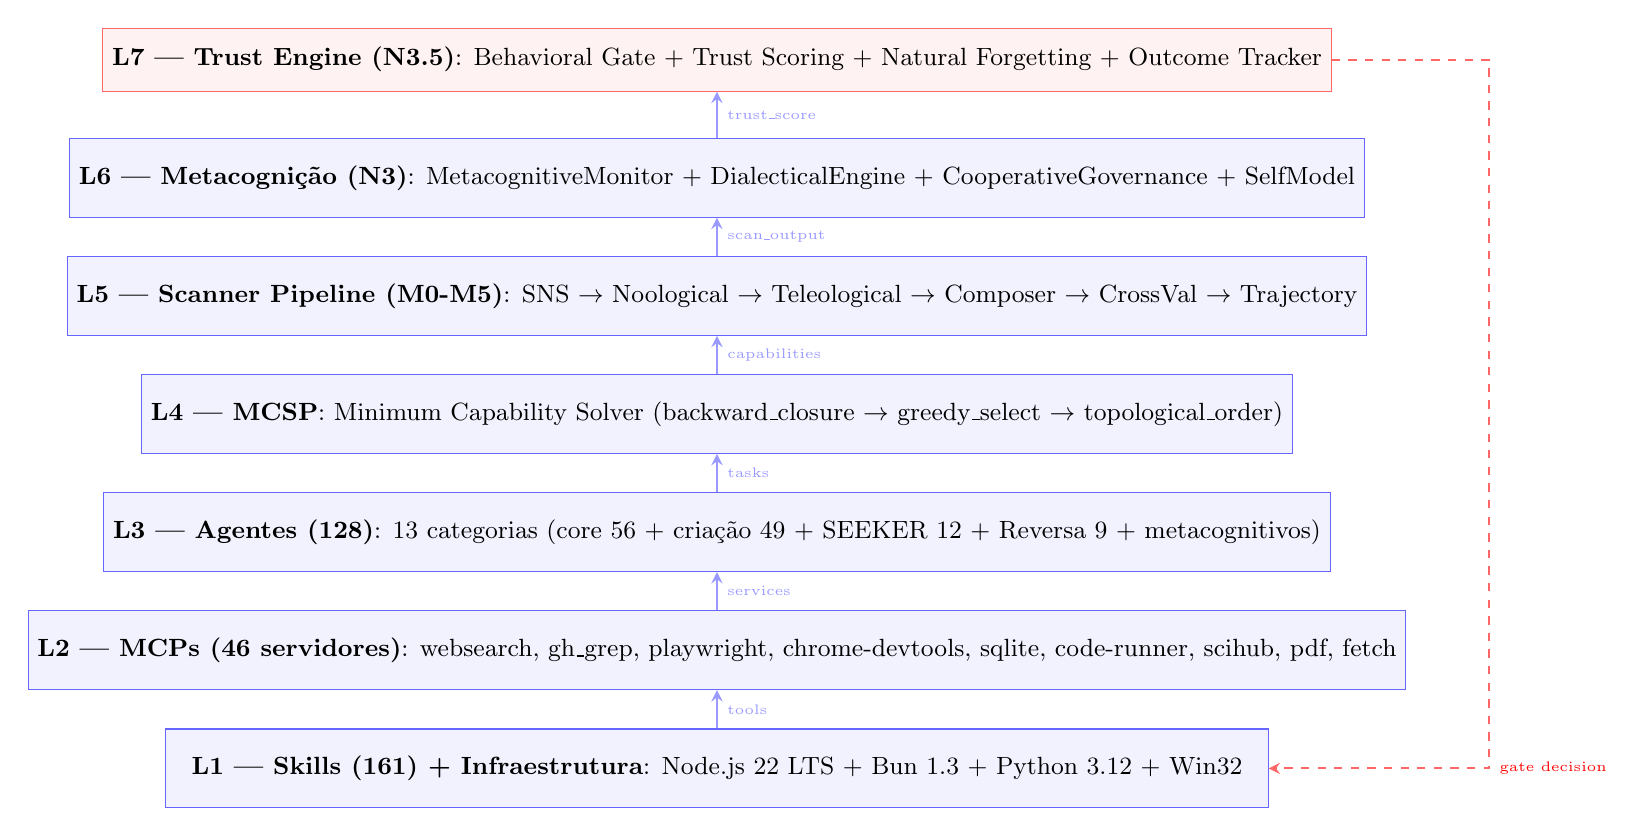
\begin{tikzpicture}[
    layer/.style={rectangle, draw=blue!60, fill=blue!5, minimum width=14cm, minimum height=1cm, align=center, font=\small},
    arrow/.style={->, >=stealth, thick, blue!40},
    gate/.style={rectangle, draw=red!60, fill=red!5, minimum width=14cm, minimum height=0.8cm, align=center, font=\small},
]
% L7 - Trust Engine
\node[gate] (L7) at (0,7) {\textbf{L7 — Trust Engine (N3.5)}: Behavioral Gate + Trust Scoring + Natural Forgetting + Outcome Tracker};
% L6 - Metacognição
\node[layer] (L6) at (0,5.5) {\textbf{L6 — Metacognição (N3)}: MetacognitiveMonitor + DialecticalEngine + CooperativeGovernance + SelfModel};
% L5 - Scanner Pipeline
\node[layer] (L5) at (0,4) {\textbf{L5 — Scanner Pipeline (M0-M5)}: SNS $\rightarrow$ Noological $\rightarrow$ Teleological $\rightarrow$ Composer $\rightarrow$ CrossVal $\rightarrow$ Trajectory};
% L4 - MCSP
\node[layer] (L4) at (0,2.5) {\textbf{L4 — MCSP}: Minimum Capability Solver (backward\_closure $\rightarrow$ greedy\_select $\rightarrow$ topological\_order)};
% L3 - Agentes
\node[layer] (L3) at (0,1) {\textbf{L3 — Agentes (128)}: 13 categorias (core 56 + criação 49 + SEEKER 12 + Reversa 9 + metacognitivos)};
% L2 - MCPs
\node[layer] (L2) at (0,-0.5) {\textbf{L2 — MCPs (46 servidores)}: websearch, gh\_grep, playwright, chrome-devtools, sqlite, code-runner, scihub, pdf, fetch};
% L1 - Skills
\node[layer] (L1) at (0,-2) {\textbf{L1 — Skills (161) + Infraestrutura}: Node.js 22 LTS + Bun 1.3 + Python 3.12 + Win32};

% Arrows between layers
\draw[arrow] (L1.north) -- (L2.south) node[midway,right,font=\tiny] {tools};
\draw[arrow] (L2.north) -- (L3.south) node[midway,right,font=\tiny] {services};
\draw[arrow] (L3.north) -- (L4.south) node[midway,right,font=\tiny] {tasks};
\draw[arrow] (L4.north) -- (L5.south) node[midway,right,font=\tiny] {capabilities};
\draw[arrow] (L5.north) -- (L6.south) node[midway,right,font=\tiny] {scan\_output};
\draw[arrow] (L6.north) -- (L7.south) node[midway,right,font=\tiny] {trust\_score};

% Gate feedback loop
\draw[arrow, red!60, dashed] (L7.east) -- ++(2,0) |- (L1.east) node[midway,right,font=\tiny,red] {gate decision};
\end{tikzpicture}
\caption{Arquitetura do OpenCode Ecosystem — 7 Camadas com Fluxo de Dados}
\label{fig:arquitetura}
\end{figure}

A Figura~\ref{fig:arquitetura} ilustra a arquitetura em 7 camadas. O fluxo de dados é ascendente: as Skills (L1) fornecem conhecimento reutilizável que é acessado pelos MCPs (L2), que por sua vez servem como ferramentas para os Agentes (L3). O MCSP (L4) recebe as capacidades identificadas pelos agentes e encontra o conjunto mínimo. O Scanner Pipeline (L5) diagnostica gaps e gera roadmaps. A Metacognição (L6) observa todo o pipeline, detecta anomalias e propõe correções. O Trust Engine (L7) atua como gate preventivo — antes de qualquer ação ser executada, o Behavioral Gate consulta o histórico de confiança (seta tracejada vermelha) e decide se a ação deve prosseguir ou ser bloqueada.
